En esta sección entraremos más en detalle en lo que a las mecánicas de \nombrejuego se refiere. Se comentarán todas las características que forman parte de la jugabilidad, y se detallarán las acciones que podrá llevar a cabo el jugador dentro de una partida típica. Además de explicar de forma concisa la organización de los menús y su utilidad.

    \section{Jugabilidad}
        \subsection{Progresión del juego}
        La progresión del juego va definida por el número de localizaciones (nuevos escenarios) desbloqueados. Al principio solo contaremos con una única localización e iremos desbloqueando las demás según resolvamos puzzles.
        
        \subsection{Progresión de la dificultad}%Challenge Structure
        %Si bien los puzzles seguirán distintos métodos para su resolución, todos los puzzles serán presentados previamente por un personaje (sea el protagonista o un PNJ).
        Cada puzzle del juego tendrán distintos métodos de resolución, ya sea uno de colocar figuras en el mapa, otro de identificación de cuadros, uno de obtener objetos, etc. Aparte de eso, la dificultad irá en aumento por la cantidad de acciones, objetos necesarios, o áreas para visitar para la resolución de dicho puzzle.
        
        \subsection{Objetivos}
        El objetivo del juego es resolver el misterio del paradero del profesor desaparecido, y por consiguiente, que el protagonista apruebe el examen suspendido. Para ello, tendrá que resolver los puzzles, uno a uno, y finalmente resolver un pequeño cuestionario con las anécdotas históricas de cada puzzle.
        
        \subsection{Flujo de juego}%Play flow
        A lo largo de esta sección, se detallará el transcurso de una partida típica a \nombrejuego. Se comentarán los pasos que ha de seguir el \emph{Jugador} desde el arranque del juego hasta completar un puzzle y pasar al siguiente nivel. De esta forma, desentrañamos el funcionamiento exacto del juego. Más adelante se definen las mecánicas y el contenido de cada pantalla.
        
        El \emph{Jugador} inicia \nombrejuego y se le presenta el \emph{Menú Principal}. Si desea iniciar una partida el \emph{Jugador} seleccionará la opción \emph{Partida nueva}, o en el caso de tener una partida ya guardada, a la opción \emph{Cargar partida} (para saber más de los menús, véase la sección ~\ref{sec:menus}).
        
        Una vez dentro del juego, veremos al personaje principal en un escenario. Dentro del cual, podremos interactuar con el escenario haciendo \emph{clicks} para ver o interactuar con sus elementos: ver lo que son, hablar con otros personajes, coger objetos, etc. Si estamos al inicio de un escenario nuevo, se sucederá una escena cinemática (de forma en la que el protagonista se mueva y hable sin requerir ninguna acción por parte del \emph{Jugador}), y un personaje de dicho escenario nos planteará un puzzle a resolver si queremos recibir una pista sobre el paradero del profesor. Según cómo hagamos dichas interacciones resolveremos el puzzle a resolver en dicho escenario y obtendremos un nuevo escenario a donde ir.
    
    %\newpage    
    \section{Controles}
        
        \begin{figure}[H] 
			\begin{center}
				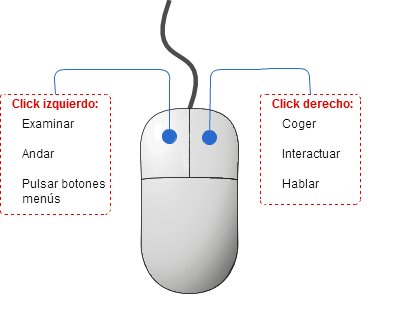
\includegraphics[scale=0.45]{controles.png}
			\end{center}
			\caption{Controles del juego}
			\label{fig:controles}
		\end{figure}
    
    %\newpage    
    \section{Mecánicas}
        
        \subsection{Movimiento}
        En esta sección definiremos cómo se moverá el personaje principal que maneja el \emph{Jugador}, además de otros movimientos tales como trasladar un objeto de sitio.
            
            \subsubsection{Movimiento general}
            Para el movimiento general del personaje principal, el jugador solo se limitará en hacer click en alguna zona donde no haya obstáculos. En el caso de que hubiera obstáculos pero fuera posible llegar desde una ruta que no sea en línea recta, el personaje principal seguirá una ruta realizada con un algoritmo A\* o similar. De esta manera el algoritmo calcula la ruta más corta desde donde esta nuestro personaje principal hasta el punto donde queremos llevarlo, y finalmente lo ejecuta para llevar a cabo el movimiento.
            
            \subsubsection{Otros movimientos}
            Los otros personajes, no se moverán o simplemente se moverán unos pasos, siento su ruta únicamente una línea recta de escasa distancia.
            
        \subsection{Objetos}
        En los escenarios en los que transcurre el juego, habrá varios objetos con los que el \emph{Jugador} podrá interactuar con ellos.
            
            \subsubsection{Describiendo objetos}
            Al mover el ratón por la pantalla, el icono del ratón cambiará a otro si está encima de un objeto. Si el \emph{Jugador} pulsa \emph{click} izquierdo, el protagonista se moverá hasta la posición más cercana a dicho objeto y le explicará al \emph{Jugador} qué es y sus impresiones propias sobre él.
            
            \subsubsection{Cogiendo objetos}
            Si el objeto es adquirible por nuestro protagonista, de la misma manera que pasamos el ratón sobre el objeto y cambia el icono del ratón al estar sobre un  objeto, en este caso hacemos \emph{click} derecho. De esta manera el protagonista se moverá hasta la posición más cercana a dicho objeto y lo cogerá, seguido de un sonido que indique el haber metido el objeto en el inventario.
            
            \subsubsection{Moviendo objetos}
            En \nombrejuego realmente no podremos mover \emph{in situ} los objetos dentro del escenario. Para poder moverlos, primero tendremos que introducir el objeto en el inventario, luego seleccionarlo dentro del inventario con \emph{click} izquierdo, y finalmente usar el objeto en el sitio concreto del escenario donde se pueda utilizar con \emph{click} derecho.
            
        \subsection{Acciones}
        Si bien casi toda las acciones se hacen de manera similar a lo descrito en la sección anterior, existen algunas diferencias que hay que puntualizarlas. Pues no todo es simplemente describir, coger y mover objetos en \nombrejuego.
        
            \subsubsection{Interruptores y botones}
            Para accionar un interruptor o botón, simplemente hay que posicionar el ratón sobre él y ver cómo cambiar el icono de este. Estando así, simplemente hay que hacer \emph{click} derecho con el ratón, el protagonista se moverá hasta donde está el interruptor o botón y lo accionará. De manera opcional, el protagonista puede decirnos si ha pasado algo en concreto al accionarlo.
            
            \subsubsection{Coger, llevar y soltar}
            En \nombrejuego solo podremos coger, llevar objetos de la manera especificada en la sección de Objetos. Soltar los objetos no será posible hasta que se hayan usado en el puzzle que los requiera.
            
            \subsubsection{Hablar}
            En el juego, podremos hablar con los otros personajes que se encuentren en el escenario. Para ello, tendremos que posicionar el ratón encima de un personaje. El icono cambiará como en las veces citadas anteriormente, y tendremos que hacer \emph{click} izquierdo. Así el protagonista se moverá a la posición más cercana que se sitúe al frente del personaje y aparecerá un diálogo entre ellos.
            
            \subsubsection{Leer}
            En \nombrejuego habrá libros y carteles para leer. La mecánica es la misma que se usa para describir un objeto, dado que los libros y carteles son objetos. 
         
	%\newpage
	\section{Inteligencia Artificial}
	En la mayoría de los videojuegos es uno de los puntos más importante, pues ella rige el comportamiento de todos los personajes, e incluso de objetos. Un enemigo que sigue una ruta y te persiga si te ve, un semáforo que cambia de luces y los coches se mueven con ello, todo esto y mucho más es gracias a las inteligencia artificial. Existen muchos y variados algoritmos para realizar distintos comportamientos dependiendo de si buscas que un personaje haga una ruta, una estrategia, o que actúen a modo de colmena los personajes que aparecen el juego, y más aún que desconozco. Sin embargo, en las aventuras gráficas no se suele hacer un gran uso de estas pues los personajes no suelen moverse de su sitio, y las conversaciones son lineales. Pero si hay un punto que a veces usa una inteligencia artificial, cuando queremos que el personaje que lleva el \emph{Jugador} se mueva en un escenario con obstáculos.
        
            \subsection{Personajes No Jugables (PNJs) o \emph{Non Player Characters} (NPCs)}
        	Si algunas veces en las aventuras gráficas aparecen PNJs enemigos que persiguen al Protagonista o amistosos que estén dando vueltas por una ruta prefijada, en el caso de \nombrejuego no va a ser así. Los PNJs se quedarán en un sitio prefijado sin moverse y solo interactuarán con el Protagonista para iniciar una conversación. 
        	
            \subsection{Jugador y sistema de colisiones}
            
            
            
	%\newpage
	    \section{Físicas}
	    El juego poseerá físicas en 2D, osease, colisiones entre planos. De esta manera, el jugador solo podrá mover su personaje sobre ciertas áreas, saber cuándo estamos pulsando encima de un objeto o personaje con el que podemos interactuar, poder acceder al menú gracias a un menú gráfico, etc.